% !Mode:: "TeX:UTF-8"
% !TEX TS-program = xelatex
\documentclass[UTF8]{report}
% \documentclass[UTF8]{report}

\usepackage[zihao=-4,heading=true]{ctex}
\usepackage{geometry}
\geometry{left=2.0cm, right=2.0cm, top=2.0cm, bottom=2.0cm}
\usepackage[colorlinks=true]{hyperref}
\usepackage{graphicx} % used for add figure to this report
\graphicspath{{img/}}
\usepackage{listings}
\usepackage{xcolor}
\usepackage{booktabs}
\usepackage[toc]{multitoc}
\usepackage{graphics}
\usepackage{subfig}
\usepackage{fancyhdr}
\usepackage{enumerate}
\usepackage[section]{placeins}


	\lstdefinestyle{customcpp}{
		numbers=left,
		numberstyle=\tiny,
		belowcaptionskip=1\baselineskip,
		breaklines=true,
		xleftmargin=\parindent,
		language=C++,
		showstringspaces=false,
		basicstyle=\footnotesize\ttfamily,
		keywordstyle=\bfseries\color{green!40!black},
		commentstyle=\itshape\color{purple!40!black},
		identifierstyle=\color{blue},
		stringstyle=\color{orange},
	}
	
	\lstdefinestyle{customjava} {
	language=Java,
	backgroundcolor=\color{lightgray},
	breaklines=true,
	% numbers=left,
	% numberstyle=\tiny,
	basicstyle=\ttfamily,
	keywordstyle=\bfseries\color{green!40!black},
	commentstyle=\itshape\color{purple!40!black},
	identifierstyle=\color{blue},
	stringstyle=\color{orange},
}	

\lstdefinestyle{myxml} {
    backgroundcolor=\color{lightgray},
	language=XML,
	breaklines=true,
    % numbers=left,
	% numberstyle=\tiny,
	basicstyle=\ttfamily,
	keywordstyle=\bfseries\color{green!40!black},
	commentstyle=\itshape\color{purple!40!black},
	identifierstyle=\color{blue},
	stringstyle=\color{orange},
}
\lstdefinestyle{mysh} {
    backgroundcolor=\color{lightgray},
	language=sh,
	breaklines=true,
    % numbers=left,
	% numberstyle=\tiny,
	basicstyle=\ttfamily,
	keywordstyle=\bfseries\color{green!40!red},
	commentstyle=\itshape\color{purple!40!black},
	identifierstyle=\color{blue},
	stringstyle=\color{orange},
}
\lstdefinestyle{mysql} {
    backgroundcolor=\color{lightgray},
	language=SQL,
	breaklines=true,
	basicstyle=\ttfamily,
	keywordstyle=\bfseries\color{green!40!red},
	commentstyle=\itshape\color{purple!40!black},
	identifierstyle=\color{blue},
	stringstyle=\color{orange},
}


\lstdefinestyle{normal} {
	language=sh,
	basicstyle=\ttfamily,
	breaklines=true,
	keywordstyle=\bfseries\color{green!40!red},
	commentstyle=\itshape\color{purple!40!black},
	identifierstyle=\color{blue},
	stringstyle=\color{orange},
}

\lstset{style=normal}

\ctexset {
part/pagestyle = empty,
chapter = {
    format = \raggedright,
    pagestyle = empty,
},
section = {
    name = {第,部分},
    number = \chinese{section},
},
subsection = {
    name = {第,节},
    number = \chinese{subsection},
}
}
\pagestyle{fancy}

\titleformat{\section}
            {\LARGE\bfseries\sffamily\color{RoyalBlue}}
            {
\includegraphics[height=2em]{hadoop/hadoop2.png} \thesection{}.}
            {1em}
            {\huge\scshape}


\begin{document}
Spark shell是一个特别适合快速开发Spark程序的工具。即使你对Scala不熟悉,仍然可以使用这个工具快速应用Scala操作Spark。
Spark shell使得用户可以和Spark集群交互,提交查询,这便于调试,也便于初学者使用Spark。
Spark shell是非常方便的,因为它很大程度上基于Scala REPL(Scala交互式shell,即Scala解释器),并继承了Scala REPL(读取-求值-打印-循环)(Read-Evaluate-Print-Loop)的所有功能。运行spark-shell,则会运行spark-submit,spark-shell其实是对spark-submit的一层封装。

下面是Spark shell的运行原理图

\begin{figure}[htbp]
    \centering
    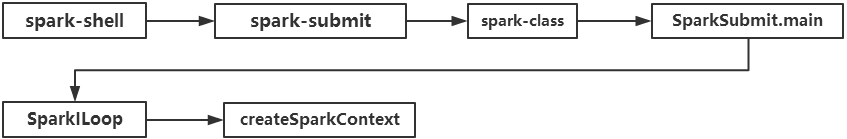
\includegraphics[width=\linewidth]{spark/spark-shell.png}    
    \caption{Spark shell的运行原理图}
    \label{fig:spark_shell}
\end{figure}
RDD有两种类型的操作 ,分别是Transformation(返回一个新的RDD)和Action(返回values)。
\begin{itemize}
    \item Transformation:根据已有RDD创建新的RDD数据集build

\begin{enumerate}[1)]
\item map(func):对调用map的RDD数据集中的每个element都使用func,然后返回一个新的RDD,这个返回的数据集是分布式的数据集。
\item filter(func) :对调用filter的RDD数据集中的每个元素都使用func,然后返回一个包含使func为true的元素构成的RDD。
\item flatMap(func):和map很像,但是flatMap生成的是多个结果。
\item mapPartitions(func):和map很像,但是map是每个element,而mapPartitions是每个partition。
\item mapPartitionsWithSplit(func):和mapPartitions很像,但是func作用的是其中一个split上,所以func中应该有index。
\item sample(withReplacement,faction,seed):抽样。
\item union(otherDataset):返回一个新的dataset,包含源dataset和给定dataset的元素的集合。
\item distinct([numTasks]):返回一个新的dataset,这个dataset含有的是源dataset中的distinct的element。
\item groupByKey(numTasks):返回(K,Seq[V]),也就是Hadoop中reduce函数接受的key-valuelist。
\item reduceByKey(func,[numTasks]):就是用一个给定的reduce func再作用在groupByKey产生的(K,Seq[V]),比如求和,求平均数。
\item sortByKey([ascending],[numTasks]):按照key来进行排序,是升序还是降序,ascending是boolean类型。
\end{enumerate}
\item  Action:在RDD数据集运行计算后,返回一个值或者将结果写入外部存储
\begin{enumerate}[1)]
\item reduce(func):就是聚集,但是传入的函数是两个参数输入返回一个值,这个函数必须是满足交换律和结合律的。
\item collect():一般在filter或者足够小的结果的时候,再用collect封装返回一个数组。
\item count():返回的是dataset中的element的个数。
\item first():返回的是dataset中的第一个元素。
\item take(n):返回前n个elements。
\item takeSample(withReplacement,num,seed):抽样返回一个dataset中的num个元素,随机种子seed。
\item saveAsTextFile(path):把dataset写到一个textfile中,或者HDFS,或者HDFS支持的文件系统中,Spark把每条记录都转换为一行记录,然后写到file中。
\item saveAsSequenceFile(path):只能用在key-value对上,然后生成SequenceFile写到本地或者Hadoop文件系统。
\item countByKey():返回的是key对应的个数的一个map,作用于一个RDD。
\item foreach(func):对dataset中的每个元素都使用func。
\end{enumerate}
\end{itemize}

\lstinputlisting[style=mysh,title=获取实验测试数据]{docs/scripts/get_data.sh}
\lstinputlisting[style=mysh,title=测试Shell操作]{docs/scripts/spark-shell-op.sh}
一些测试过程中的效果截图:

\begin{center}
    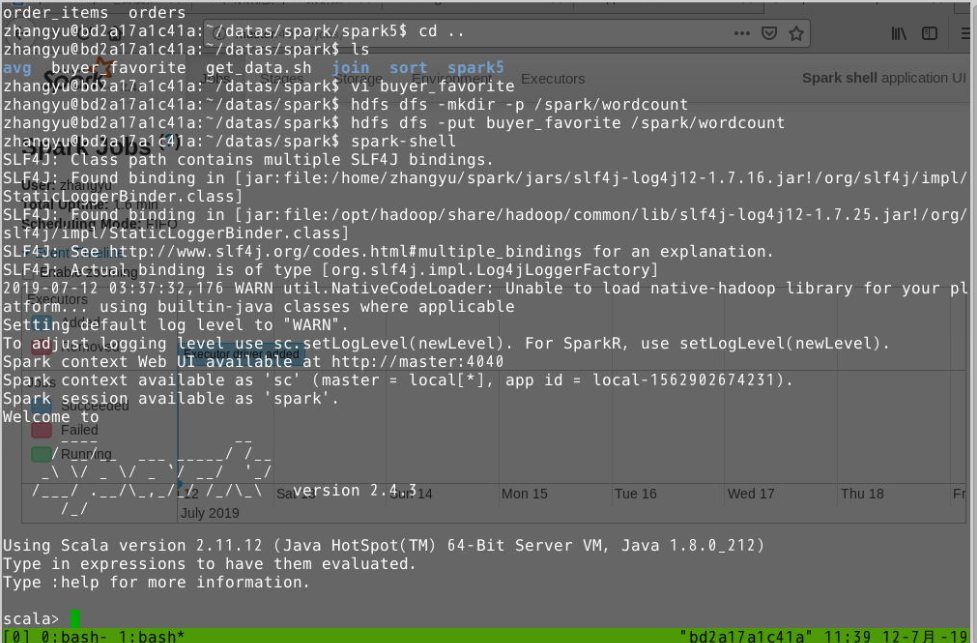
\includegraphics[width=\linewidth]{spark/spark-shell2.png}    
\end{center}
    
\begin{center}
    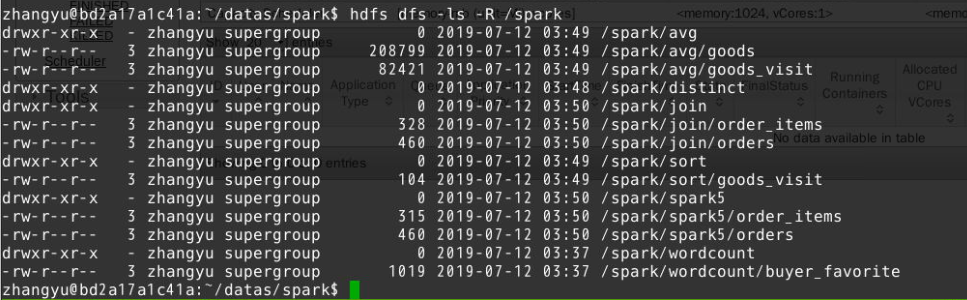
\includegraphics[width=\linewidth]{spark/test_data.png}
\end{center}

\lstinputlisting[style=mysh,title=buyer\_favorite]{docs/scripts/buyer_favorite}

\begin{center}
    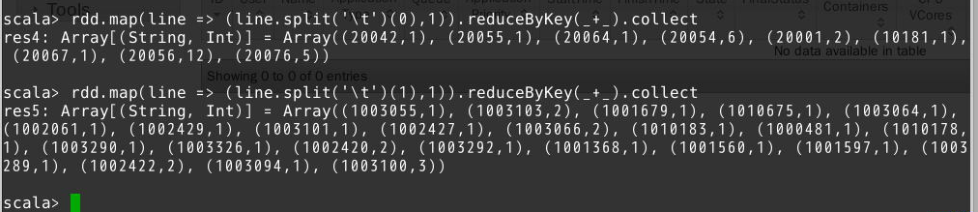
\includegraphics[width=\linewidth]{spark/wordcount.png}

    Spark实现WordCount,比Hadoop要简单的多
\end{center}
    
\begin{center}
    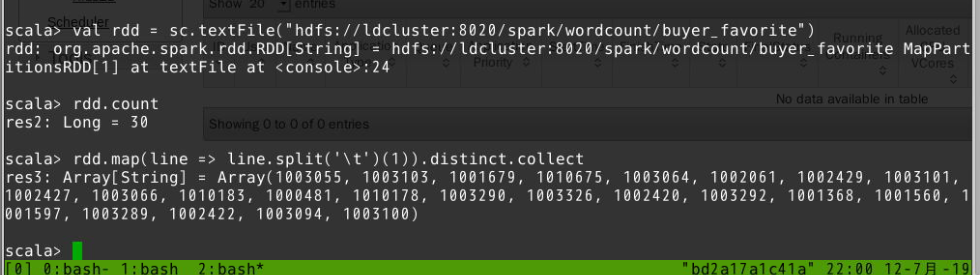
\includegraphics[width=\linewidth]{spark/rdd2.png}

    Spark实现去重,查看哪些商品被收藏
\end{center}
    
\lstinputlisting[style=mysh,title=goods\_visit]{docs/scripts/goods_visit}

\begin{center}
    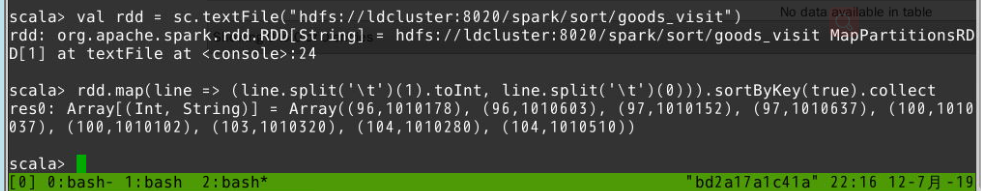
\includegraphics[width=\linewidth]{spark/rddsort.png}

    Spark对用户记录进行排序,实现按购买数升序排列。
\end{center}
    
\lstinputlisting[style=mysh,title=orders]{docs/scripts/orders}

\lstinputlisting[style=mysh,title=order\_items]{docs/scripts/order_items}

\begin{center}
    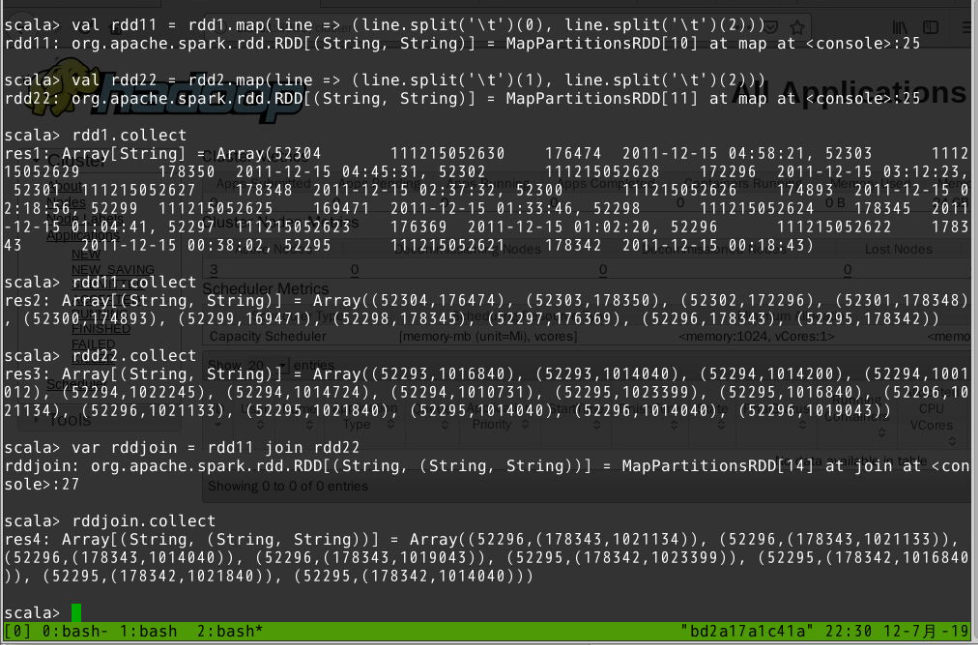
\includegraphics[width=\linewidth]{spark/rddjoin.png}

    Spark实现两张表的Join操作
\end{center}
\end{document}